
\par
Wszystkie elementy wyświetlające dane z pliku \DICOM dziedziczą po klasie \sokarclass{SceneIndicator}.
Diagram klas UML znajduje się na rysunku \ref{uml:sokar-scene-indicators}.

\begin{figure}[!htbp]
    \centering
    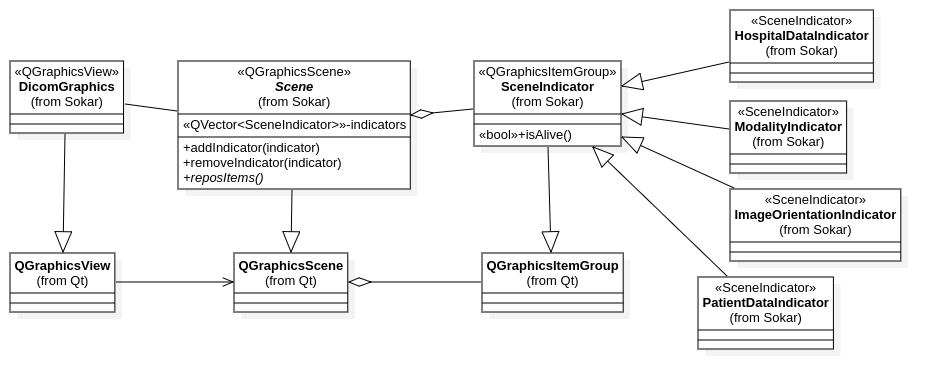
\includegraphics[width=\textwidth]{img/uml/dicom-scene-indicators.png}
    \caption{Diagram klas UML dziedziczenia klasy \sokarclass{DicomScene}.}
    \label{uml:sokar-scene-indicators}
\end{figure}

\par
Domyślnie obiekty wyświetlające informacje (tytuły punktów to nazwy klas):
\paragraph{Dane pacjenta}

Są implementowane przez \sokarclass{PatientDataIndicator}.
Pojawia się zawsze na scenie w lewym górnym rogu i zawiera następujące linie:
\begin{itemize}
    \item Nazwa pacjenta oraz płeć

          Nazwa pacjenta znajduje się w \dicomtag{PatientName}{0010}{0010} o \dicomvr{PN}.

          Płeć, zapisana jest w \dicomtag{PatientSex}{0010}{0040} i może mieć następujące wartości:
          \begin{itemize}
              \item \dataword{M } --- oznacza mężczyznę, wyświetlana jako O
              \item \dataword{F } --- oznacza kobietę, wyświetlana jako O
              \item \dataword{O } --- oznacza inną płeć i nie jest wyświetlana
          \end{itemize}

          W przypadku określenia inne płci niż jest w standardzie bądź braku tagu płeć nie będzie widoczna.

          Przykład: \dataword{Adam Jędrzejowski O}.

    \item Identyfikator pacjenta

          Unikalny identyfikator pacjenta z tagu \dicomtag{PatientID}{0010}{0020} wyświetlane w takiej formie jakiej jest zapisane, bez żadnej obróbki.
          W praktyce najczęściej jest to numer z systemu używanego w danym szpitalu, rzadziej numer PESEL.

          Przykład: \dataword{HIS/000000}.

    \item Data urodzenia oraz wiek pacjenta w trakcie badania

          Data urodzenia znajdująca się w \dicomtag{PatientBirthDate}{0010}{0030} i jest zamieniana na format \dataword{YYYY-MM-DD}.
          Dodatkowo, jeżeli tag \dicomtag{PatientAge}{0010}{1010} jest obecny, wyświetlany jest także wiek pacjenta w czasie badania.

          Przykład: \dataword{born 1982-08-09, 28 years}.

    \item Opis wykonany przez instytucję opis lub klasyfikację badania (komponentu)

          Tekst brany z \dicomtag{StudyDescription}{0008}{1030} i wyświetlany bez żadnej obróbki.

          UWAGA: Ta wartość jest wpisywana przez technika, operatora lub lekarza wykonującego badanie, więc wartość ta może być nie przewidywalna.

    \item Opis serii

          Tekst brany z \dicomtag{SeriesDescription}{0008}{103E} i wyświetlany bez żadnej obróbki.

          UWAGA: Ta wartość jest wpisywana przez technika, operatora lub lekarza wykonującego badanie, więc wartość ta może być nie przewidywalna.
\end{itemize}

Przykład pełnego teksu:

\texttt{\\
    \textbf{Adam Jędrzejowski} O\\
    HIS/123456\\
    born 1996-07-16, 19 years\\
    Kregoslup ledzwiowy a-p + boczne\\
    AP
}

\paragraph{Dane jednostki organizacyjnej}

Są implementowane przez \sokarclass{HospitalDataIndicator}.
Pojawia się zawsze na scenie w prawym górnym rogu i zawiera następujące linie:
\begin{itemize}
    \item Nazwa instytucji

          Tekst brany z \dicomtag{InstitutionalDepartmentName}{0008}{1040} i wyświetlany bez żadnej obróbki.

\end{itemize}

\paragraph{Orientacja obrazu}

\par
Jest implementowana przez \sokarclass{ImageOrientationIndicator}.
Obiekt wyświetlający cztery litery oznaczające orientacje obrazu w stosunku do pacjenta.
Obiekt posiada cztery pola: lewe, górne, prawe i dolne.

\par
Każda z sześciu możliwych liter oznacza kierunek oraz zwrot w jakim jest ułożony pacjent:
\begin{itemize}
    \item \dataword{R} --- right --- część prawa pacjenta
    \item \dataword{L} --- left --- część
    \item \dataword{A} --- anterior --- przód pacjenta
    \item \dataword{P} --- posterior --- tył pacjenta
    \item \dataword{F} --- feet --- część dolna
    \item \dataword{H} --- head --- część górna
\end{itemize}

\par
Pełeny opis implementacji algorytmu wyznaczania stron znajduje się w sekcji \label{sec:algorithm-imageorientationindicator}.

\paragraph{Podziałka}

Jest implementowana przez \sokarclass{PixelSpacingIndicator}.
Obiekt wyświetlający podziałkę informującą jakich rzeczywistych rozmiarów jest obiekt na obrazie, pojawia się na dole i po prawie stronie sceny, gdy znacznik \dicomtag{PixelSpacing}{0028}{0030} jest obecny.
Wygląd podziałki można zaobserwować na rysunku \ref{fig:imageorientationindicator1}.

Podziałka dostosowuje swoją wielkość do obecnej sceny, jak i do innych elementów na scenie.
Wartości wyświetlane biorą pod uwagę transformatę skali i rotacji obrazu.

\paragraph{Dodatkowe informacje o modalności}

Są implementowane przez \sokarclass{ModalityIndicator}.
Obiekt wyświetla informacje o akwizycji obrazu.
Dane różnią się w zależności od modalności obrazu.
Domyślnie zawierają następujące linie:
\begin{itemize}
    \item bla bla bla
    \item bla bla bla
    \item bla bla bla
    \item bla bla bla
\end{itemize}

W przypadku następujących modalności zawierają również następujące informacje:
\begin{itemize}
    \item bla bla bla
    \item bla bla bla
    \item bla bla bla
    \item bla bla bla
\end{itemize}